Test orig: \cite{LimZD13}.

We use the random decision forest framework implemented in the toolbox of Piotr Doll\'ar~\cite{Dollar2013toolbox}.

Check capitals: \cite{Arbelaez09}. % these are one after the other
Arxiv: \cite{Hallman2014}

Dollar's: \cite{Dollar2014fast,DollarICCV13edges}

Reference with question mark: \cite{Fowlkes04}.

% \begin{figure}[ht!]
%  \centering
%  \subfigure[Input image]{%
%  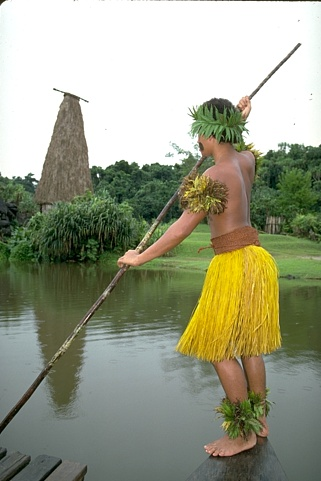
\includegraphics[width=0.3\textwidth]{images/examples/hawaii/arbelaez2011-035.png}
% \label{fig:subfigure1}}
%  \subfigure[Edge map]{%
%  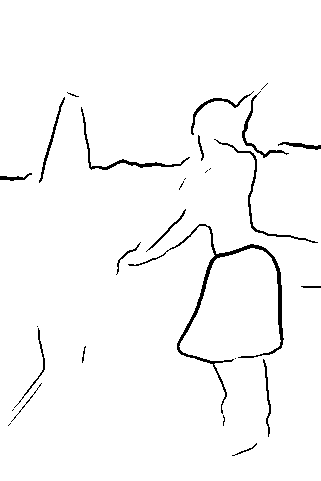
\includegraphics[width=0.3\textwidth]{images/examples/hawaii/edge_map_arbelaez2011-039.png}
% \label{fig:subfigure2}}
% \subfigure[Probability of boundary]{%
%  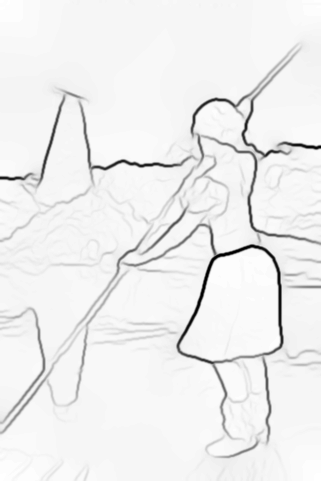
\includegraphics[width=0.3\textwidth]{images/examples/hawaii/Pb_arbelaez2011-039.png}
% \label{fig:subfigure3}}
% % \quad
% % \qquad
% % \caption[Caption that doesn't show?]{{\bf Boundary detection} (courtesy~\cite{Arbelaez11}).}
% \caption{Referencing subfigure: \protect\subref{fig:subfigure2} some text \protect\subref{fig:subfigure1} some other text}
% \label{fig:bdry_detection}
% \end{figure}
% 
% % simple figure, no labels
% \begin{figure}[ht!]
%  \centering
%  \subfigure[Input image]{%
%  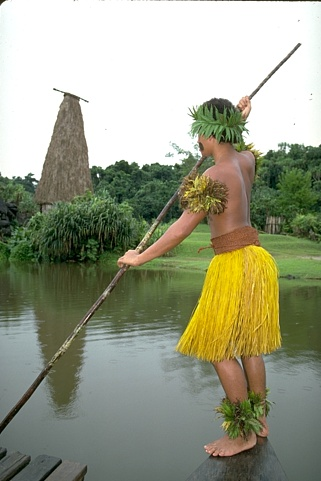
\includegraphics[width=0.3\textwidth]{images/examples/hawaii/arbelaez2011-035.png}
%  }
%  \subfigure[Edge map]{%
%  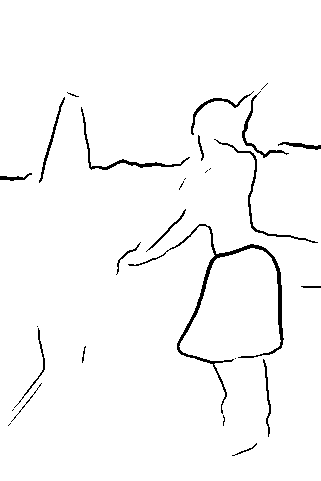
\includegraphics[width=0.3\textwidth]{images/examples/hawaii/edge_map_arbelaez2011-039.png}
%  }
% \subfigure[Probability of boundary]{%
%  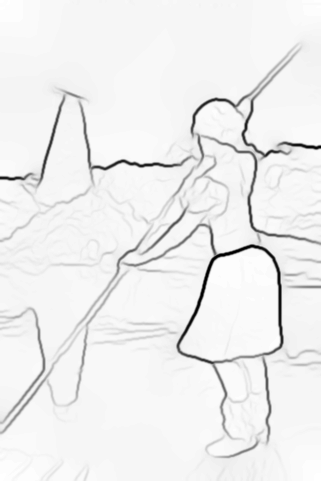
\includegraphics[width=0.3\textwidth]{images/examples/hawaii/Pb_arbelaez2011-039.png}
%  }
%  \caption[Caption that doesn't show?]{
%   {\bf Boundary detection} (courtesy~\cite{Arbelaez11}).}
% \end{figure}